\documentclass{article}
\usepackage[top=2in, bottom=1in, left=1in, right=1in]{geometry}
\usepackage{fancyhdr}
\usepackage{amsmath}
\pagestyle{fancyplain}
\usepackage{Sweave}
\begin{document}
\lhead{Math 571B\\ Homework 1}
\rhead{Brian Mannakee\\ \today}

\Sconcordance{concordance:Homework1.tex:Homework1.Rnw:%
1 4 1 1 0 4 1 1 15 4 1 1 2 31 0 1 2 5 1}


\begin{enumerate}
  \item
    \begin{enumerate}
      \item The randomization matrix for treatments A and B along with the means and mean difference for each of the 20 unique possible designs 
% latex table generated in R 2.15.1 by xtable 1.7-1 package
% Tue Jan 29 20:54:19 2013
\begin{table}[ht]
\centering
\begin{tabular}{r|lllllllll}
  \hline
 & 1 & 2 & 3 & 4 & 5 & 6 & MeanA & MeanB & MeanDiff \\ 
  \hline
Yield & 3 & 5 & 4 & 2 & 7 & 4 & 0.00 & 0.00 & 0.00 \\ 
  Design 1 & A & B & B & A & B & A & 3.00 & 5.33 & 2.33 \\ 
  Design 2 & A & B & B & A & A & B & 4.00 & 4.33 & 0.33 \\ 
  Design 3 & A & B & A & B & A & B & 4.67 & 3.67 & -1.00 \\ 
  Design 4 & A & A & B & B & A & B & 5.00 & 3.33 & -1.67 \\ 
  Design 5 & A & A & B & B & B & A & 4.00 & 4.33 & 0.33 \\ 
  Design 6 & A & B & A & B & B & A & 3.67 & 4.67 & 1.00 \\ 
  Design 7 & A & B & B & B & A & A & 4.67 & 3.67 & -1.00 \\ 
  Design 8 & B & A & B & B & A & A & 5.33 & 3.00 & -2.33 \\ 
  Design 9 & B & A & B & A & B & A & 3.67 & 4.67 & 1.00 \\ 
  Design 10 & B & A & A & B & B & A & 4.33 & 4.00 & -0.33 \\ 
  Design 11 & B & A & A & B & A & B & 5.33 & 3.00 & -2.33 \\ 
  Design 12 & B & A & B & A & A & B & 4.67 & 3.67 & -1.00 \\ 
  Design 13 & A & B & A & A & B & B & 3.00 & 5.33 & 2.33 \\ 
  Design 14 & A & A & B & A & B & B & 3.33 & 5.00 & 1.67 \\ 
  Design 15 & A & A & A & B & B & B & 4.00 & 4.33 & 0.33 \\ 
  Design 16 & B & A & A & A & B & B & 3.67 & 4.67 & 1.00 \\ 
  Design 17 & B & B & A & A & B & A & 3.33 & 5.00 & 1.67 \\ 
  Design 18 & B & B & A & B & A & A & 5.00 & 3.33 & -1.67 \\ 
  Design 19 & B & B & A & A & A & B & 4.33 & 4.00 & -0.33 \\ 
  Design 20 & B & B & B & A & A & A & 4.33 & 4.00 & -0.33 \\ 
   \hline
\end{tabular}
\caption{Randomization Matrix}
\end{table}      \item The mean difference between treatments in Design 1, the actual experiment, is $2.33$. There are a total of 4 experiments out of twenty that have a mean absolute difference greater than or equal to $2.33$. So the p-value, calculated as $Pr(|Difference| \ge 2.33 | randomization) = \frac{4}{20} = .20$.
      \item For the two-sample t-test with $H_0: \mu_a = \mu_b$ vs. $H_a: \mu_b \ne \mu_a$, the t statistic is -2.214 and the p-value is 0.102
      \item The two-sided two-sample t-test gives a smaller p-value than the randomization test, most likely because of the small sample size for each treatment.
    \end{enumerate}
  \item[2.15]
    \begin{enumerate}
      \item We need to test the hypothesis that the population mean $\mu$ is greater than $\mu_0 = 120$. The Hypotheses are $H_0: \mu \le 120$ vs. $H_a: \mu > 120$. We will use the t-test, rejecting the null if
          $$t_0 = \frac{\bar{y} - \mu_0}{S/\sqrt{n}} > t_{\alpha,n-1}$$
      \item Here $\bar{y}$ = 131, $S =$ 19.545, and $n=10$. Therefore $t_0 =$ 1.78. According to the table in the appendix of Montgomery, $t_{0.01,9} = 2.821$. Since $t_0$ is less than $t_{0.01,9}$ we can not reject the null hypothesis at the $1\%$ level.
      \item $t_{0.05,9} = 1.833$ and $t_{0.10,9} = 1.833$ so the actual p-value lies between .05 and .10, but much closer to .05. According to R it is 0.054.
      \item The $99\%$ confidence interval is given by formula 2.38 in Montgomery
        $$\begin{array}{rcl}P(\bar{y} - t_{.01/2,n-1}*S/\sqrt{n} &\le& \mu \le \bar{y} + t_{.01/2,n-1}*S/\sqrt{n}) = .01 \\
                          P(131 - 3.25*19.545/\sqrt{10} &\le& \mu \le 131 + 3.25*19.545/\sqrt{10}) = .01 \\
                          P(131 - 20.087 &\le& \mu \le 131+ 20.087) = .01 \\
                          P(110.93 &\le& \mu \le 151.087) =.01
        \end{array}$$
    \end{enumerate}
  \item[2.16] We can evaluate the normality assumption by constructing a QQ plot.
        \begin{figure}[h]
          \begin{center}
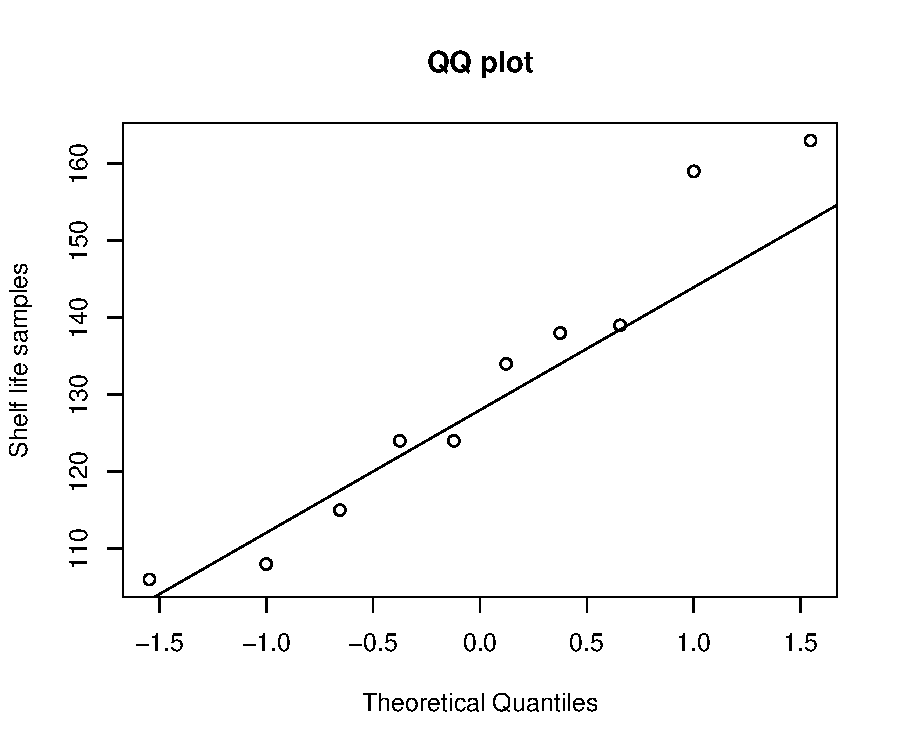
\includegraphics{Homework1-003}
          \end{center}
        \end{figure}
            
            Subjectively, based on the small sample provided, it appears reasonable to conclude that the shelf life of the population is normally distributed. If this assumption were substantially violated, the t-test would not be valid, and another way would have to be found to estimate the mean shelf life. 
  \item[2.24] I will use the R function t.test to generate numbers in this question (a)-(e).
    \begin{enumerate}
      \item The two-sample t-statistic for this sample, testing the hypothesis $H_0: \mu_{95} > \mu_{100}$ vs. $H_a:\mu_{95} \le \mu_{100}$ is 2.675 while $t_{0.05,14}$ is 1.761. Thus we have can not reject the null, that higher temperatures provide lower mean photoresist thickness, at the 5\% level.
      \item The actual p-value for this two-sample t-test is 0.009
      \item Pr(0.854 $\le \mu_{100}-\mu_{95} \le \inf$) = .05. There is a 95\% probability that the difference between the mean photoresist thickness is greater than 0.854 kA.
      \item The figures below show that the mean photoresist thickness at 95 degrees is generally greater than that for 100 degrees, visually verifying our previous result. 
              \begin{figure}[h]
          \begin{center}
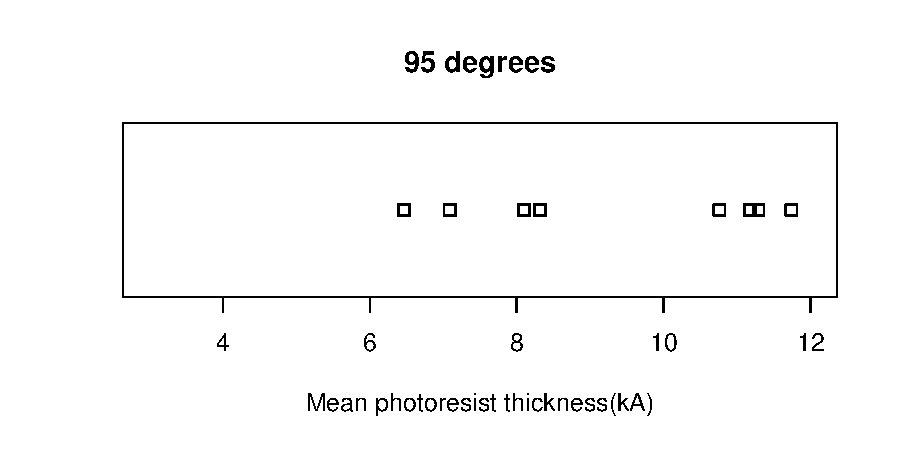
\includegraphics{Homework1-004}
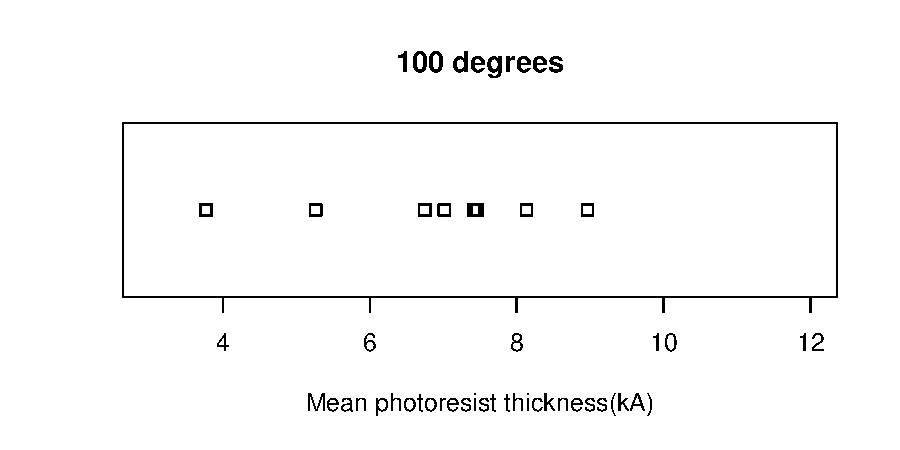
\includegraphics{Homework1-005}
          \end{center}
        \end{figure}\newpage
      \item We will test the normality assumption using a QQ plot as in 2.16.
              \begin{figure}[h]
          \begin{center}
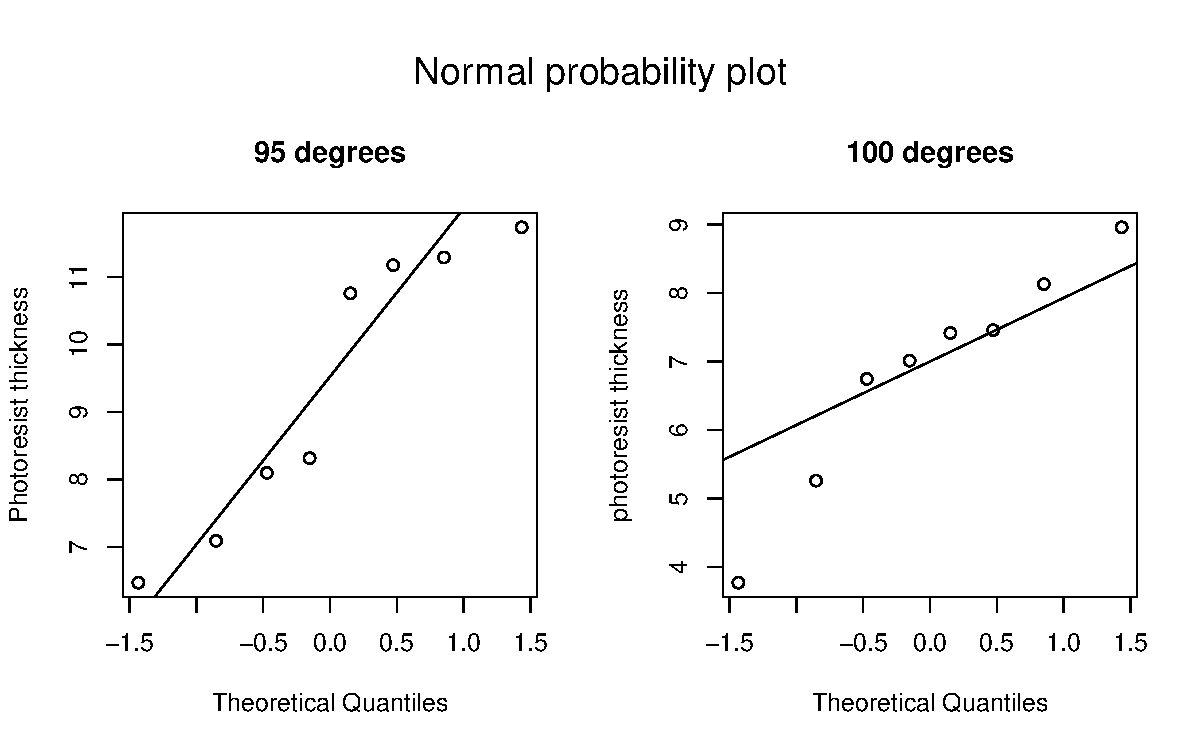
\includegraphics{Homework1-006}
          \end{center}
        \end{figure}
        
        The normality assumption is justified by the data, although the two low values at 100 degrees seem to diverge from normal.
      \item Using the pooled sample variance $S_p^2 = \frac{(n_1-1)S_1^2 + (n_2-1)S_2^2}{n_1 + n_2 -2} = $ 3.55, the effect size for a 2.5kA mean difference is $d = \frac{2.5}{2*\sqrt{3.55}} = $ 0.663. Using $n=16$ the R function pwr.t.test gives power = $\beta$ = 0.443. With the current sample size of 16 there is a 44.3\% chance of rejecting $H_0:\mu_{95}\ne \mu_{100}$ when it is false.
      \item Using the same pooled variance as above, $d = \frac{1.5}{2*\sqrt{3.55}}=$ 0.398. To detect an effect that size with a power of 90\% you need a total sample size of $n^*=$ 134, so each treatment will need to be sampled $\frac{n^*+1}{2} \approx$ 67.5 times, which we round up to $n_1 = n_2 = 68$.
    \end{enumerate}
  \item[2.27] I will use the R function t.test to generate numbers in this problem.
    \begin{enumerate}
      \item There is not a significant difference in means between the populations the samples were drawn from at the $\alpha = 0.05$ level.
      \item The two sample t-test for $H_0: \mu_1 = \mu_2$ has a p=value of 0.522 at the $\alpha = 0.05$ level.
      \item The 95\% confidence interval for the mean difference in mean diameter measurements is \\ -0.00092 $ < \mu_1-\mu_2 < $ 0.00175.
    \end{enumerate}
\end{enumerate}



\end{document}
